\documentclass[11pt]{article}

%================================================================
%================================================================
%
%                           Preamble
%
%================================================================
%================================================================

%======================================================
%
%                      Packages
%
%======================================================

\usepackage[margin=1in]{geometry}  % set the margins to 1in
\usepackage{graphicx}              % to include figures
\usepackage{amsmath}               % great math stuff
\usepackage{amsfonts}              % for blackboard bold, etc
\usepackage{amsthm}                % better theorem environments
\usepackage{titlesec}              % format section titles

\usepackage{soul}
\usepackage{mathrsfs}
\usepackage{enumerate}
\usepackage{multicol}
\usepackage[makeroom]{cancel}
\usepackage{xcolor}
%\usepackage[usenames,dvipsnames]{color}
\usepackage{tikz}
\usepackage{setspace}
\usepackage{pdfpages}
\usepackage{listings}
\usepackage{matlab-prettifier}
\usepackage{xspace}
\usepackage{multirow}

\usepackage{amssymb}
\usepackage{parskip}
\usepackage{color}
\usepackage[hyphens]{url}
\usepackage{latexsym}
\usepackage{fancyhdr}
\usepackage{fancyvrb}
\usepackage{algpseudocode}
\usepackage{verbatim}
\usepackage{collectbox}
\usepackage{scrextend}
\usepackage{array}
\usetikzlibrary{arrows.meta,shapes,calc}

\DeclareMathOperator{\id}{id}

%======================================================
%
%                   New Commands
%
%======================================================

\newcommand{\bd}[1]{\mathbf{#1}}  % for bolding symbols
\newcommand{\RR}{\mathbb{R}}      % for Real numbers
\newcommand{\ZZ}{\mathbb{Z}}      % for Integers
\newcommand{\col}[1]{\left[\begin{matrix} #1 \end{matrix} \right]}
\newcommand{\comb}[2]{\binom{#1^2 + #2^2}{#1+#2}}
\newcommand{\overfrac}[2]{\genfrac{}{}{0pt}{}{#1}{#2}}

\newcommand{\numdash}{\nobreakdash--}
\newcommand{\blank}[1]{\underline{\hspace{#1}}}
\newcommand{\N}{\ensuremath{\mathbb{N}}}
\newcommand{\Z}{\ensuremath{\mathbb{Z}}}
\newcommand{\Q}{\ensuremath{\mathbb{Q}}}
\newcommand{\R}{\ensuremath{\mathbb{R}}}
\newcommand{\C}{\ensuremath{\mathbb{C}}}
\newcommand{\B}{\ensuremath{\mathbb{B}}}
\newcommand{\T}{\ensuremath{\mathbb{T}}}
\newcommand{\Tau}{\ensuremath{\mathcal{T}}}
\newcommand{\HS}{\ensuremath{\mathcal{H}}}
\newcommand{\intom}{\ensuremath{\int_{\Omega}}}
\newcommand{\fa}{\ensuremath{\ \forall\ }}
\newcommand{\ex}{\ensuremath{\ \exists\ }}
\newcommand{\idty}{{\mathchoice {\rm 1\mskip-4mu l} {\rm 1\mskip-4mu l} %
    {\rm 1\mskip-4.5mu l} {\rm 1\mskip-5mu l}}}
\newcommand{\MATLAB}{\textsc{Matlab}\xspace}
\newcommand{\norm}[1]{\left\lVert#1\right\rVert}

\newtheorem{proposition}{Proposition}[section]
\newtheorem{lemma}[proposition]{Lemma}
\newtheorem{theorem}[proposition]{Theorem}
\newtheorem{corollary}[proposition]{Corollary}
\newtheorem{conjecture}[proposition]{Conjecture}
\theoremstyle{definition}
\newtheorem{definition}[proposition]{Definition}
\newtheorem{example}[proposition]{Example}
\theoremstyle{remark}
\newtheorem{remark}[proposition]{Remark}
\newtheorem{claim}[proposition]{Claim}
\newtheorem{notation}[proposition]{Notation}

\def\Xint#1{\mathchoice
	{\XXint\displaystyle\textstyle{#1}}%
	{\XXint\textstyle\scriptstyle{#1}}%
	{\XXint\scriptstyle\scriptscriptstyle{#1}}%
	{\XXint\scriptscriptstyle\scriptscriptstyle{#1}}%
	\!\int}
\def\XXint#1#2#3{{\setbox0=\hbox{$#1{#2#3}{\int}$ }
		\vcenter{\hbox{$#2#3$ }}\kern-.6\wd0}}
\def\ddashint{\Xint=}
\def\dashint{\Xint-}

\makeatletter
\newcommand{\mybox}{%
	\collectbox{%
		\setlength{\fboxsep}{1pt}%
		\fbox{\BOXCONTENT}%
	}%
}
\makeatother

\newcommand{\newquestion}{\hrulefill\vspace{-0.8\baselineskip}\\\null\hrulefill\vspace{-1.0\baselineskip}}
\newcommand{\newpart}{\vspace{-0.5\baselineskip}\hrulefill\vspace{-1.3\baselineskip}}

\DeclareMathOperator{\ran}{ran}
\DeclareMathOperator{\krnl}{ker}
\DeclareMathOperator{\dist}{dist}
\DeclareMathOperator{\image}{im}
\DeclareMathOperator{\supp}{supp}
\DeclareMathOperator{\vol}{vol}
\DeclareMathOperator{\spn}{span}
\DeclareMathOperator{\GL}{GL}
\DeclareMathOperator{\card}{card}
\DeclareMathOperator{\LCM}{LCM}
\DeclareMathOperator{\HCF}{HCF}

%\numberwithin{equation}{chapter}

%======================================================
%
%                   Format Specifications
%
%======================================================

\everymath{\displaystyle}
\setlength\parindent{0pt}
\titleformat{\section}{\normalfont}{\thesection}{}{}
\titleformat{\subsection}{\normalfont}{\thesubsection}{}{}
\titleformat{\subsubsection}{\normalfont}{\thesubsubsection}{}{}
\theoremstyle{plain}

\lstset{
  numbers=left,
  numberstyle=\scriptsize,
  stepnumber=1,
  numbersep=8pt,
  showstringspaces=false,
  breaklines=true,
  frame=single
}

%================================================================
%================================================================
%
%                          Homework 3
%
%================================================================
%================================================================
\begin{document}
  \begin{flushright}
    Mikhail Gaerlan\\
    21 February 2018\\
    MAT 226B Freund
  \end{flushright}
\vspace{-1.3\baselineskip}


\newquestion
%======================================================
%
%                    Problem 1
%
%======================================================
\section*{Problem 1}

\newpart
%--------------------------
%    Problem 1 Part A
%--------------------------
\subsection*{(a)}
Let $x_j=hj$, $y_k=hk$, and $h=1/\left(m+1\right)$ for $j,k=1,\dots,m$, and let $b_{0j}=b_0\left(x_j\right)$, $b_{1j}=b_1\left(x_j\right)$, $c_{0k}=c_0\left(y_k\right)$, and $c_{1k}=c_1\left(y_j\right)$. To include the boundary conditions, we include new matrices $B\in\R^{m\times m}$ and $C\in\R^{m\times m}$ such that
\begin{equation*}
  B=\left[
    \begin{array}{cccc}
      b_{01}&b_{02}&\cdots&b_{0m}\\
      0&0&\cdots&0\\
      \vdots&\vdots&&\vdots\\
      0&0&\cdots&0\\
      b_{11}&b_{12}&\cdots&b_{1m}\\
    \end{array}
  \right]\qquad C=\left[
  \begin{array}{ccccc}
    c_{01}&0&\cdots&0&c_{11}\\
    c_{02}&0&\cdots&0&c_{12}\\
    \vdots&\vdots&&\vdots&\vdots\\
    c_{0m}&0&\cdots&0&c_{1m}\\
  \end{array}
  \right].
\end{equation*}
Then, $T_mV+VT_m-B-C=h^2F$, so
\begin{eqnarray*}
  F'&=&Z^T\left(h^2F+B+C\right)Z\\
  v_{jk}'&=&\frac{f_{jk}'}{\lambda_j+\lambda_k},\quad\textrm{for all }j,k=1,2,\dots,m\\
  V&=&ZV'Z^T
\end{eqnarray*}

\newpart
%--------------------------
%    Problem 1 Part B
%--------------------------
\subsection*{(b)}
\lstinputlisting[style=Matlab-editor,basicstyle=\ttfamily\small]{../Code/solvePoisson.m}

\newpart
%--------------------------
%    Problem 1 Part C
%--------------------------
\subsection*{(c)}
\begin{eqnarray*}
  v\left(x,0\right)&=&b_0\left(x\right)=0\\
  v\left(x,1\right)&=&b_1\left(x\right)=\sin\left(\beta\pi x\right)\cos\left(\gamma \pi\right)\\
  v\left(0,y\right)&=&c_0\left(y\right)=0\\
  v\left(1,y\right)&=&c_1\left(y\right)=y^\alpha\sin\left(\beta\pi\right)\cos\left(\gamma\pi y\right)\\
  \frac{\partial v\left(x,y\right)}{\partial x}&=&\beta\pi y^\alpha\sin\left(\beta\pi x\right)\sin\left(\gamma\pi y\right)\\
  \frac{\partial^2v\left(x,y\right)}{\partial x^2}&=&-\beta^2\pi^2y^\alpha\sin\left(\beta\pi x\right)\cos\left(\gamma\pi y\right)\\
  \frac{\partial v\left(x,y\right)}{\partial y}&=&\alpha  y^{\alpha -1} \sin (\beta  \pi  x) \cos (\gamma  \pi  y)-\gamma  \pi  y^{\alpha} \sin (\beta  \pi  x) \sin (\gamma  \pi  y)\\
  \frac{\partial^2v\left(x,y\right)}{\partial y^2}&=&\alpha  (\alpha -1) y^{\alpha -2} \sin (\beta  \pi  x) \cos (\gamma  \pi  y)-\alpha \gamma  \pi  y^{\alpha -1} \sin (\beta  \pi  x) \sin (\gamma  \pi  y)\\
                   &&-\gamma  \pi \alpha  y^{\alpha -1} \sin (\beta  \pi  x) \sin (\gamma  \pi  y)-\gamma ^2 \pi ^2 y^{\alpha } \sin (\beta  \pi  x) \cos (\gamma  \pi  y)\\
  f\left(x,y\right)&=&\beta^2\pi^2y^\alpha\sin\left(\beta\pi x\right)\cos\left(\gamma\pi y\right)-\alpha  (\alpha -1) y^{\alpha -2} \sin (\beta  \pi  x) \cos (\gamma  \pi  y)\\
                   &&+2\alpha \gamma  \pi  y^{\alpha -1} \sin (\beta  \pi  x) \sin (\gamma  \pi  y)+\gamma ^2 \pi ^2 y^{\alpha } \sin (\beta  \pi  x) \cos (\gamma  \pi  y)
\end{eqnarray*}

\newpart
%--------------------------
%    Problem 1 Part D
%--------------------------
\subsection*{(d)}
\lstinputlisting[style=Matlab-editor,basicstyle=\ttfamily\small]{../Code/homework3_1_d_1.m}
\begin{tabular}{ccc}
  case&$m$&\texttt{error}\\\hline
  \begin{tabular}{r}
    i)\\
    ii)\\
    iii)\\
    iv)\\
    v)\\
  \end{tabular}&$\begin{array}{r}
\texttt{27}\\
\texttt{68}\\
\texttt{53}\\
\texttt{58}\\
\texttt{86}\\
\end{array}
$&$\begin{array}{r}
\texttt{4.728617202247598e-04}\\
\texttt{4.988921326820606e-04}\\
\texttt{4.837994973282411e-04}\\
\texttt{4.914479216866496e-04}\\
\texttt{4.983532030559124e-04}\\
\end{array}
$
\end{tabular}
\begin{center}
  \begin{tabular}{|>{\centering\arraybackslash}r|m{4.3cm}|m{4.3cm}|m{4.3cm}|}
    \hline
    case&right-hand side& actual & approximation\\\hline
    i)&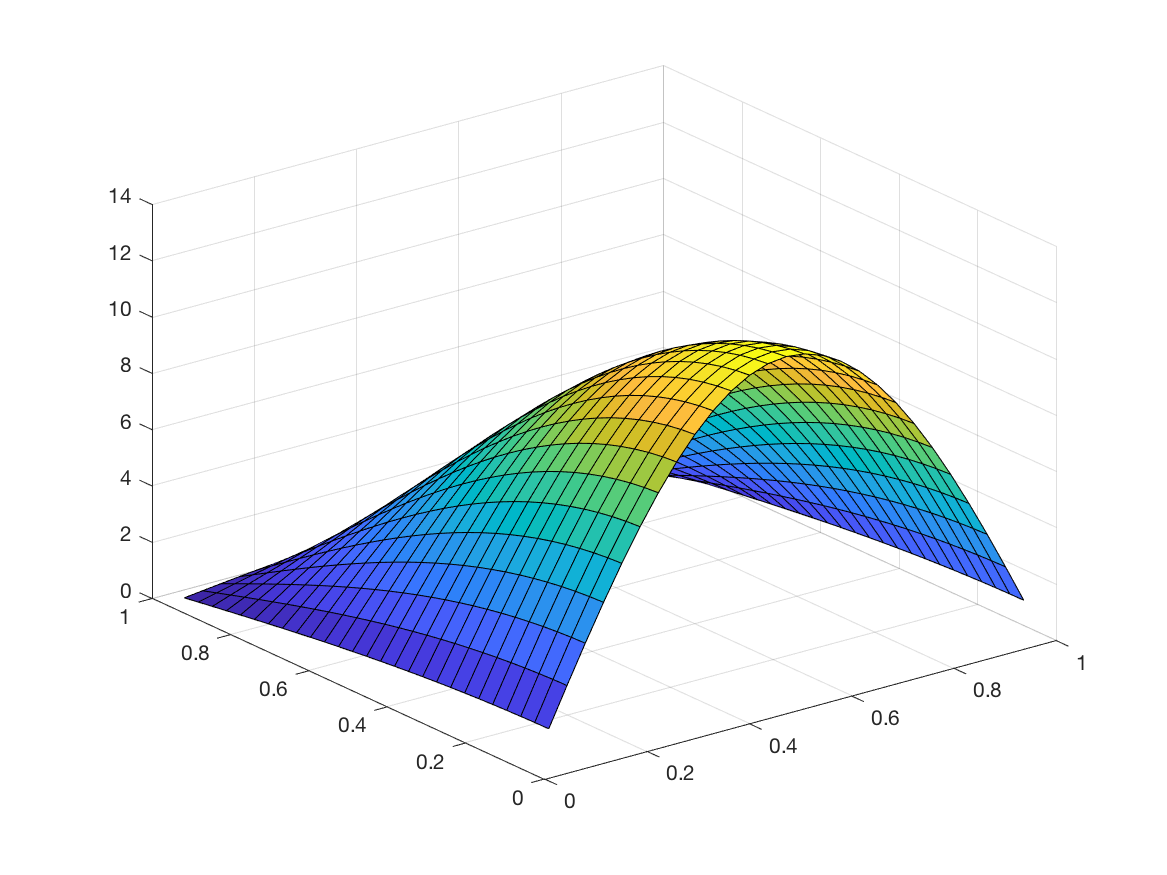
\includegraphics[width=\linewidth]{../Figures/poisson_rhs_1.png}&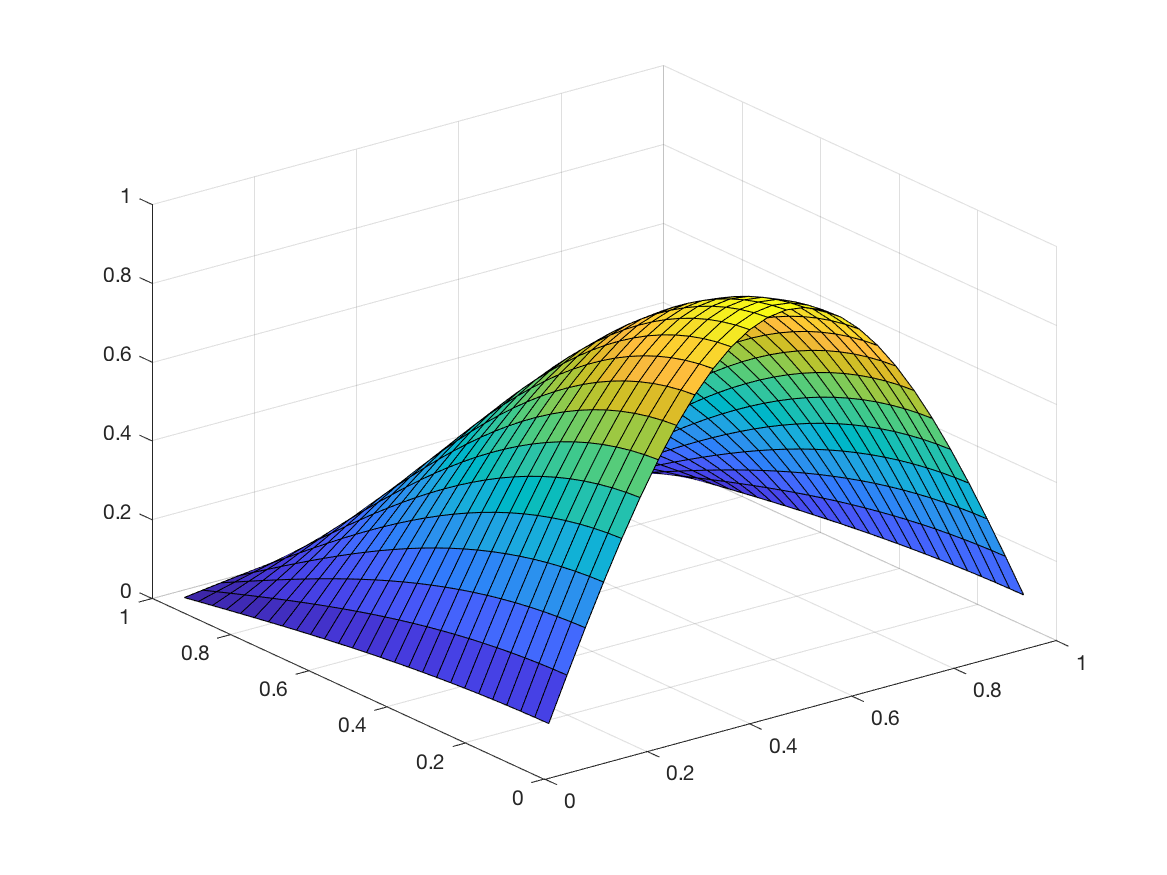
\includegraphics[width=\linewidth]{../Figures/poisson_actual_1.png}&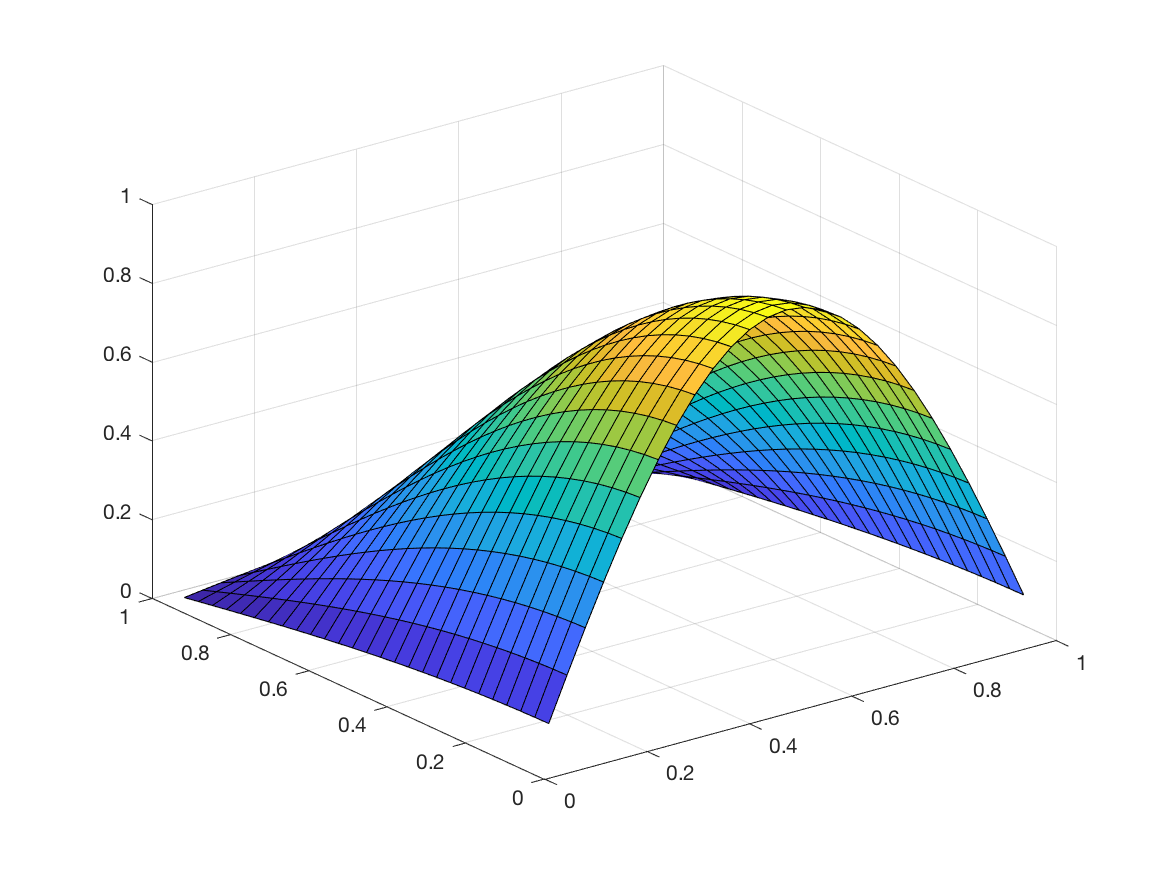
\includegraphics[width=\linewidth]{../Figures/poisson_approx_1.png}\\\hline
    ii)&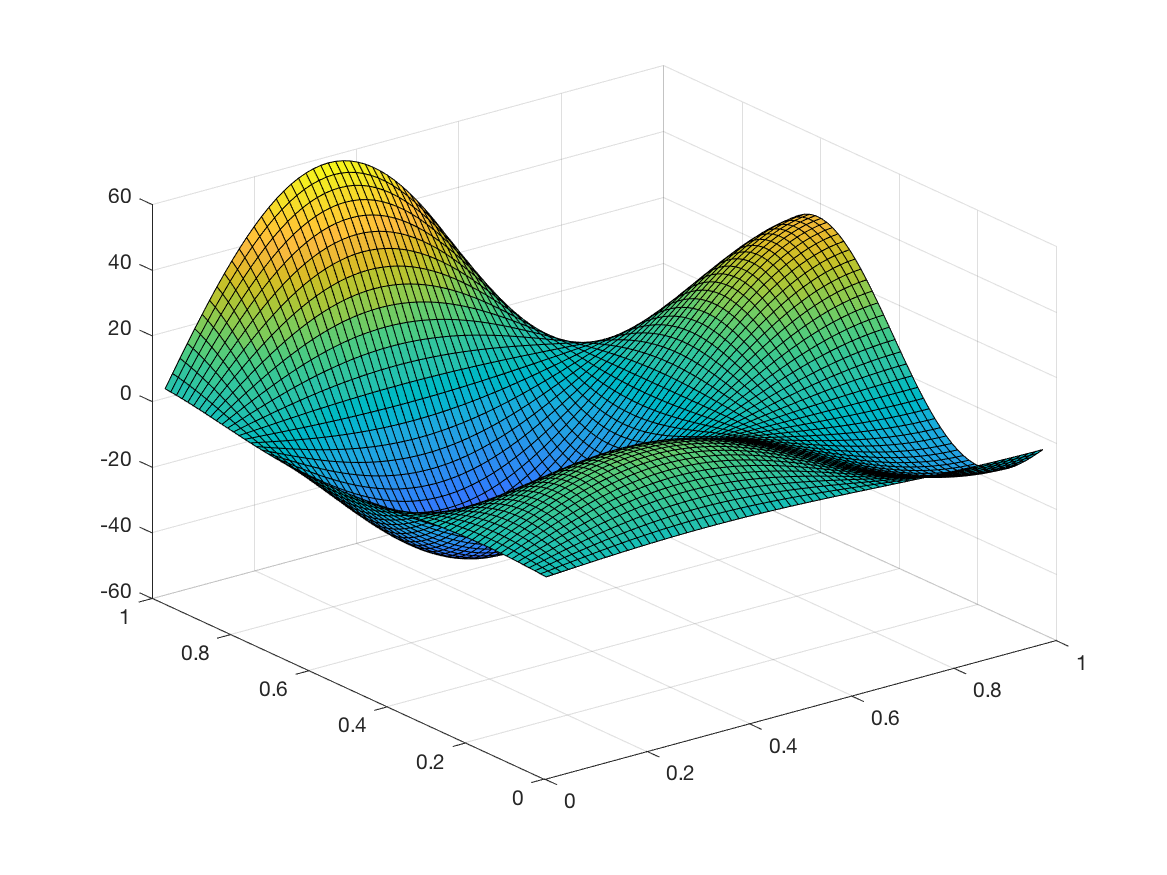
\includegraphics[width=\linewidth]{../Figures/poisson_rhs_2.png}&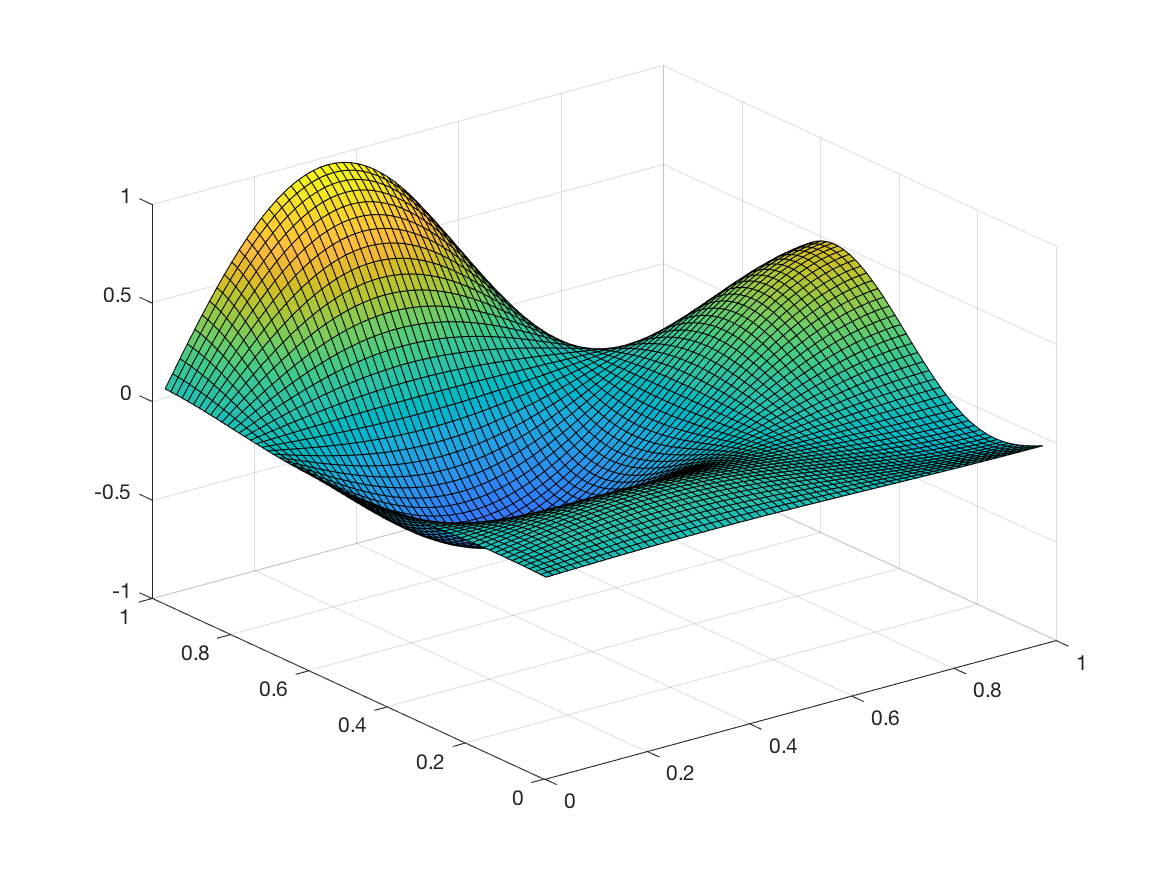
\includegraphics[width=\linewidth]{../Figures/poisson_actual_2.png}&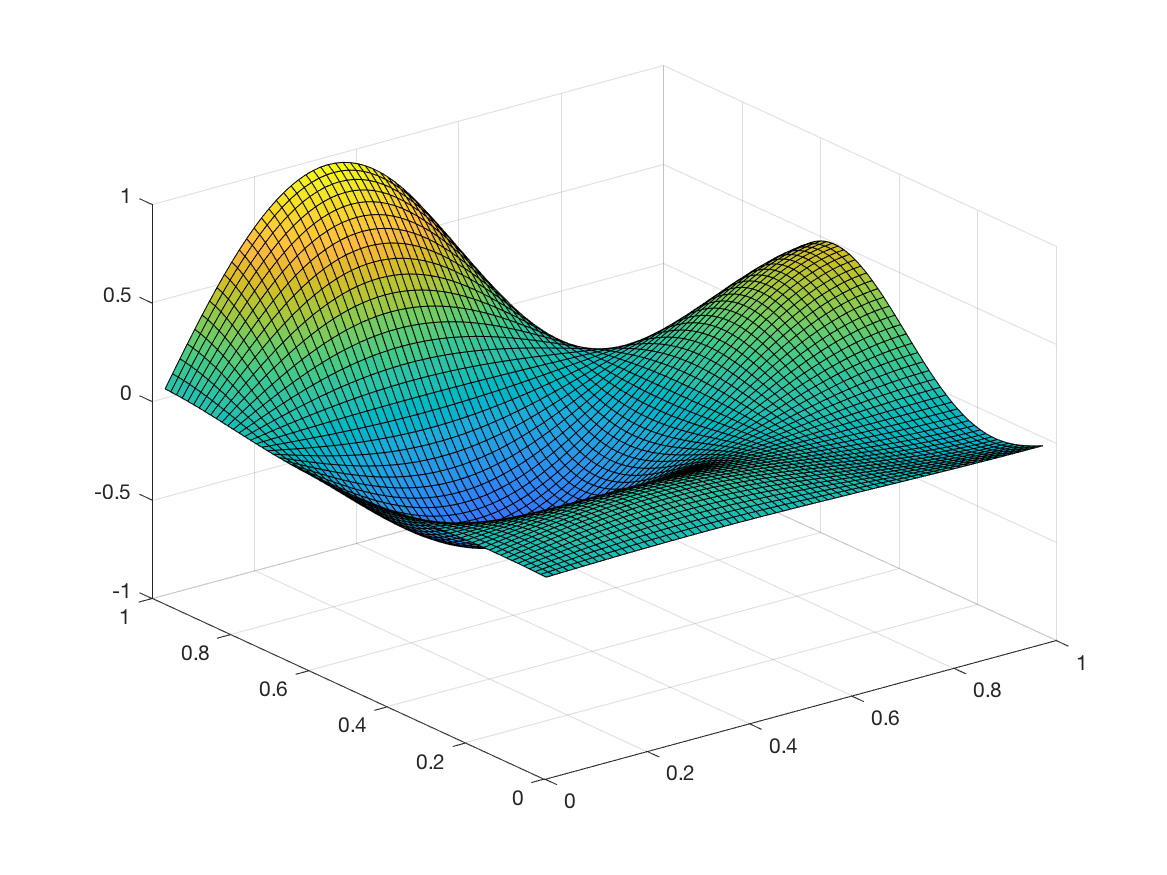
\includegraphics[width=\linewidth]{../Figures/poisson_approx_2.png}\\\hline
    iii)&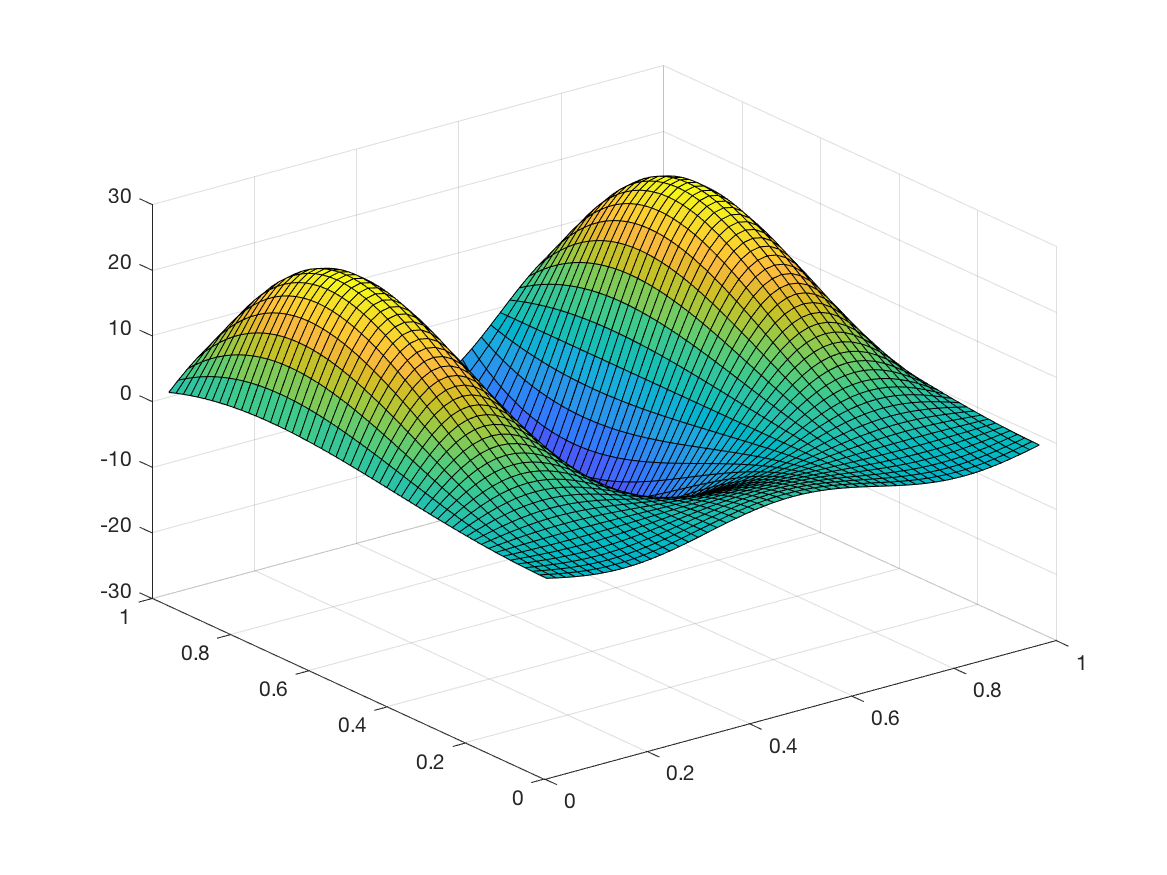
\includegraphics[width=\linewidth]{../Figures/poisson_rhs_3.png}&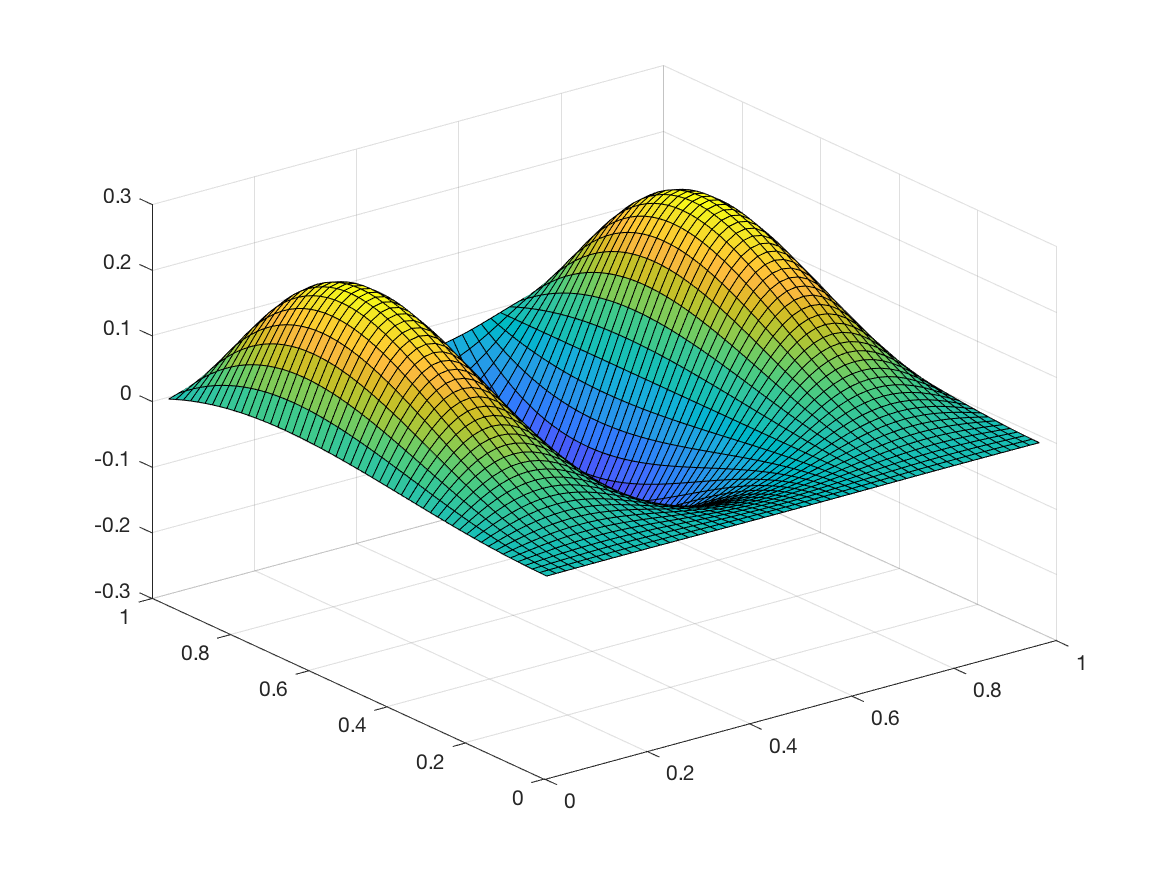
\includegraphics[width=\linewidth]{../Figures/poisson_actual_3.png}&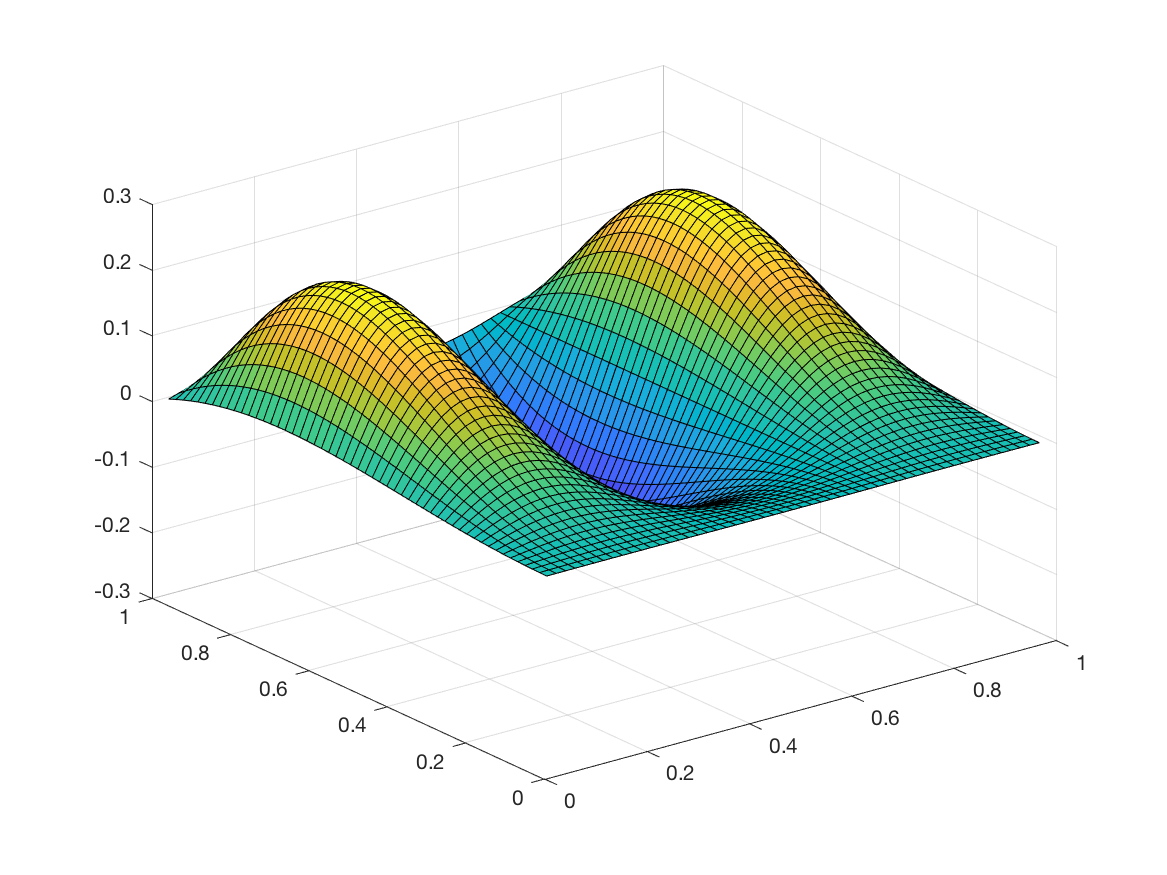
\includegraphics[width=\linewidth]{../Figures/poisson_approx_3.png}\\\hline
    iv)&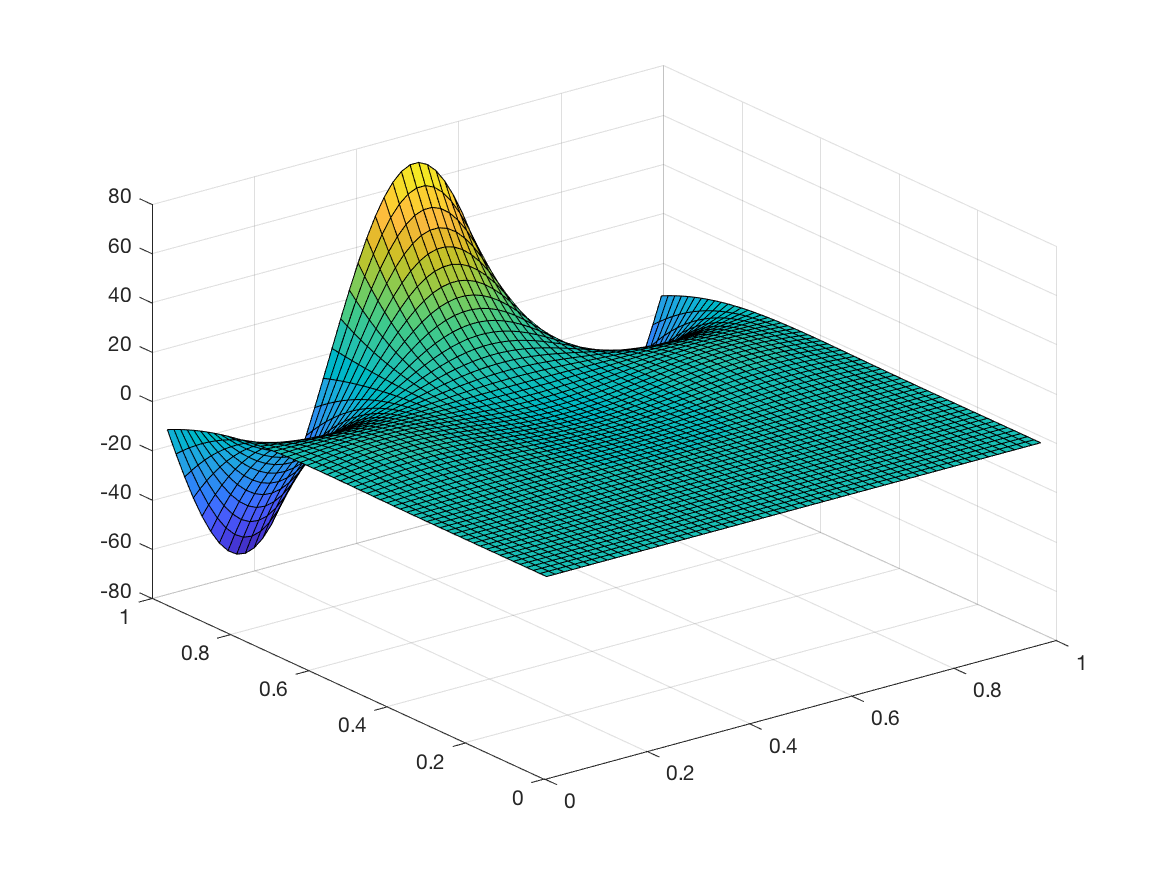
\includegraphics[width=\linewidth]{../Figures/poisson_rhs_4.png}&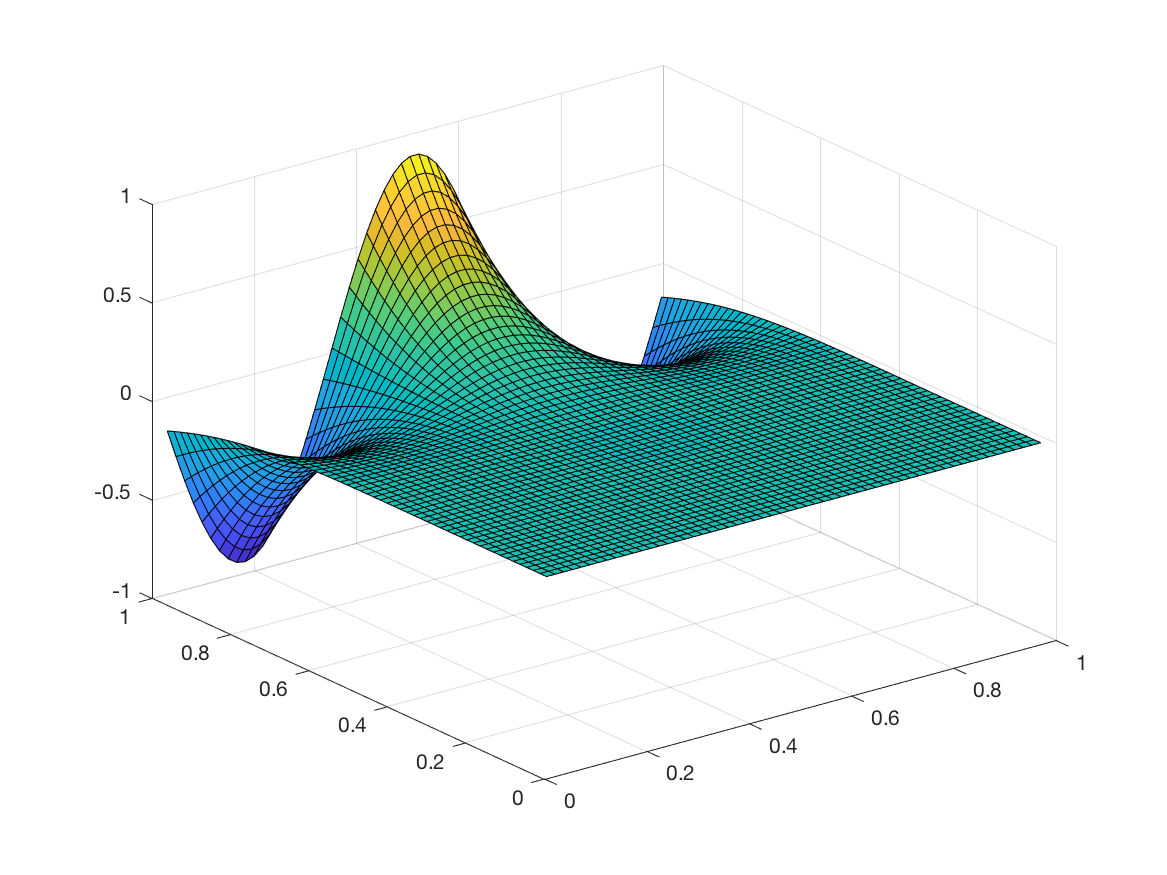
\includegraphics[width=\linewidth]{../Figures/poisson_actual_4.png}&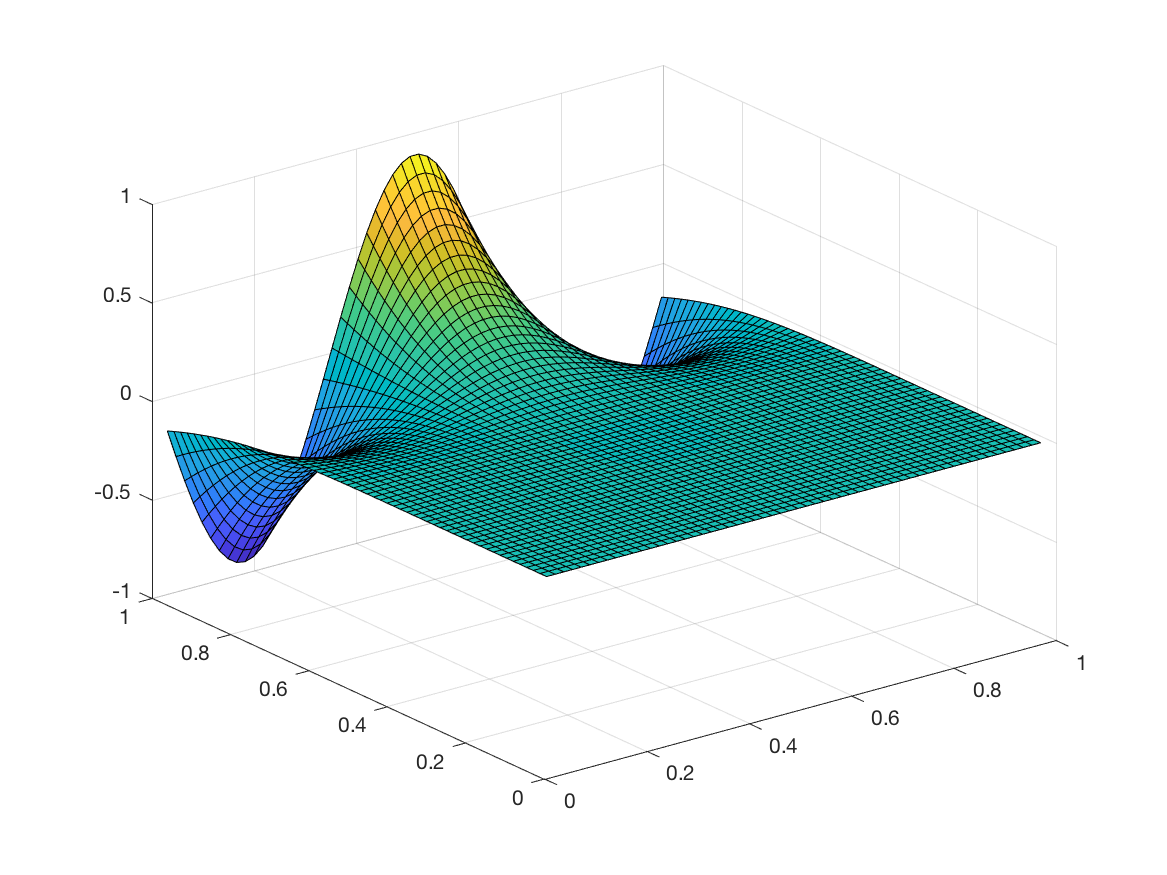
\includegraphics[width=\linewidth]{../Figures/poisson_approx_4.png}\\\hline
    v)&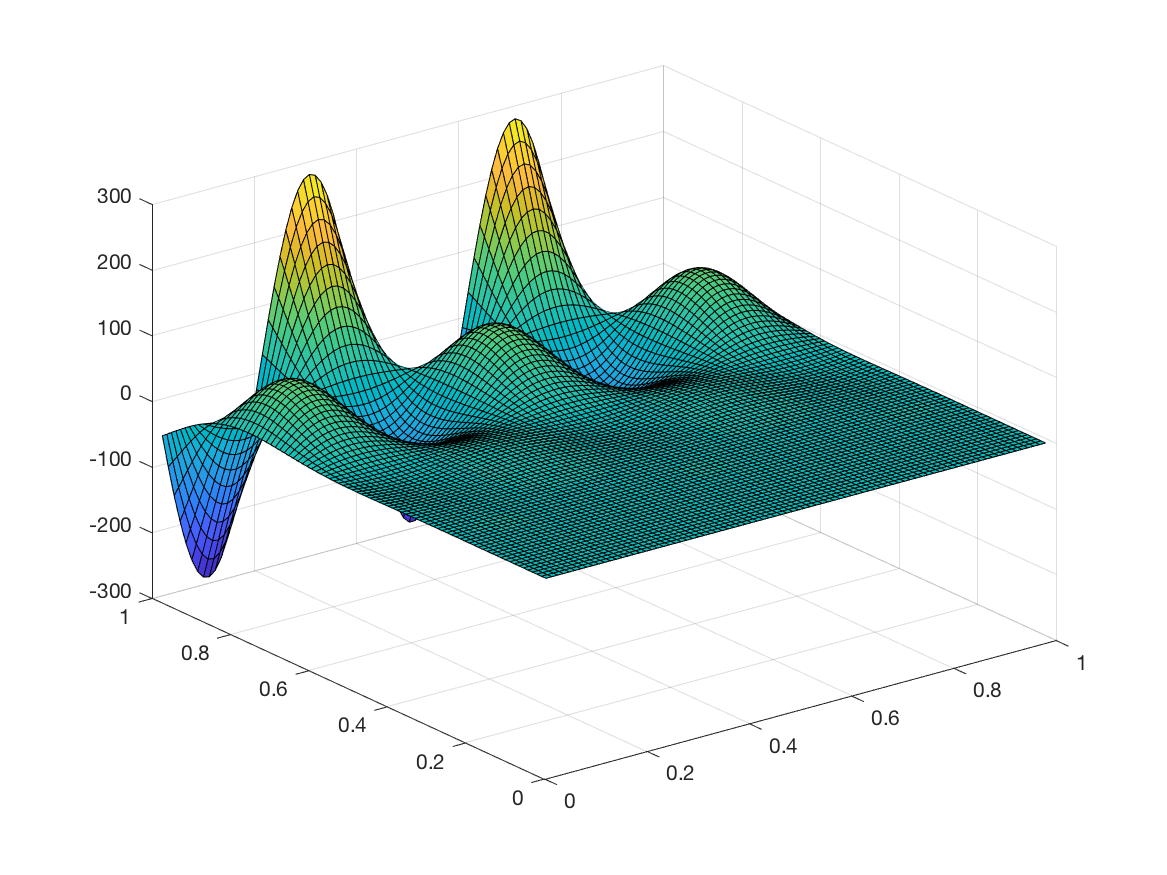
\includegraphics[width=\linewidth]{../Figures/poisson_rhs_5.png}&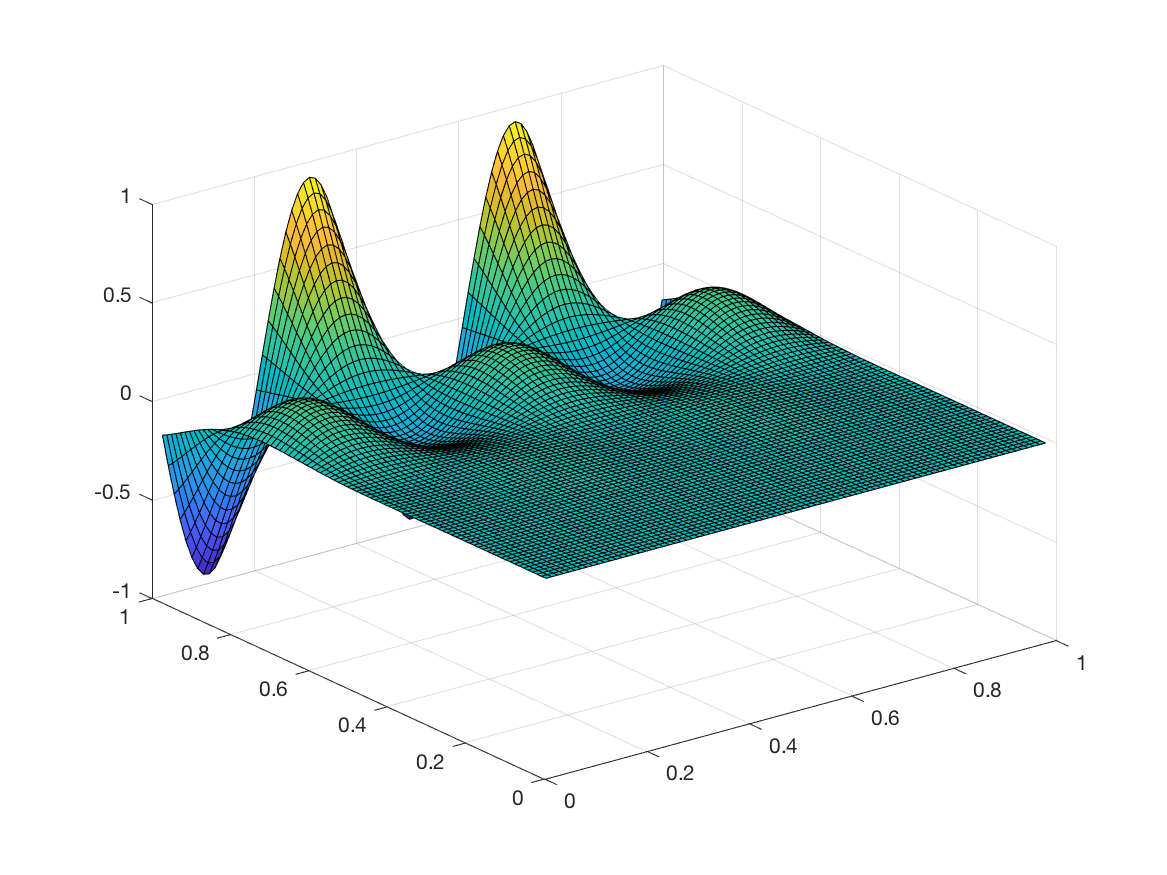
\includegraphics[width=\linewidth]{../Figures/poisson_actual_5.png}&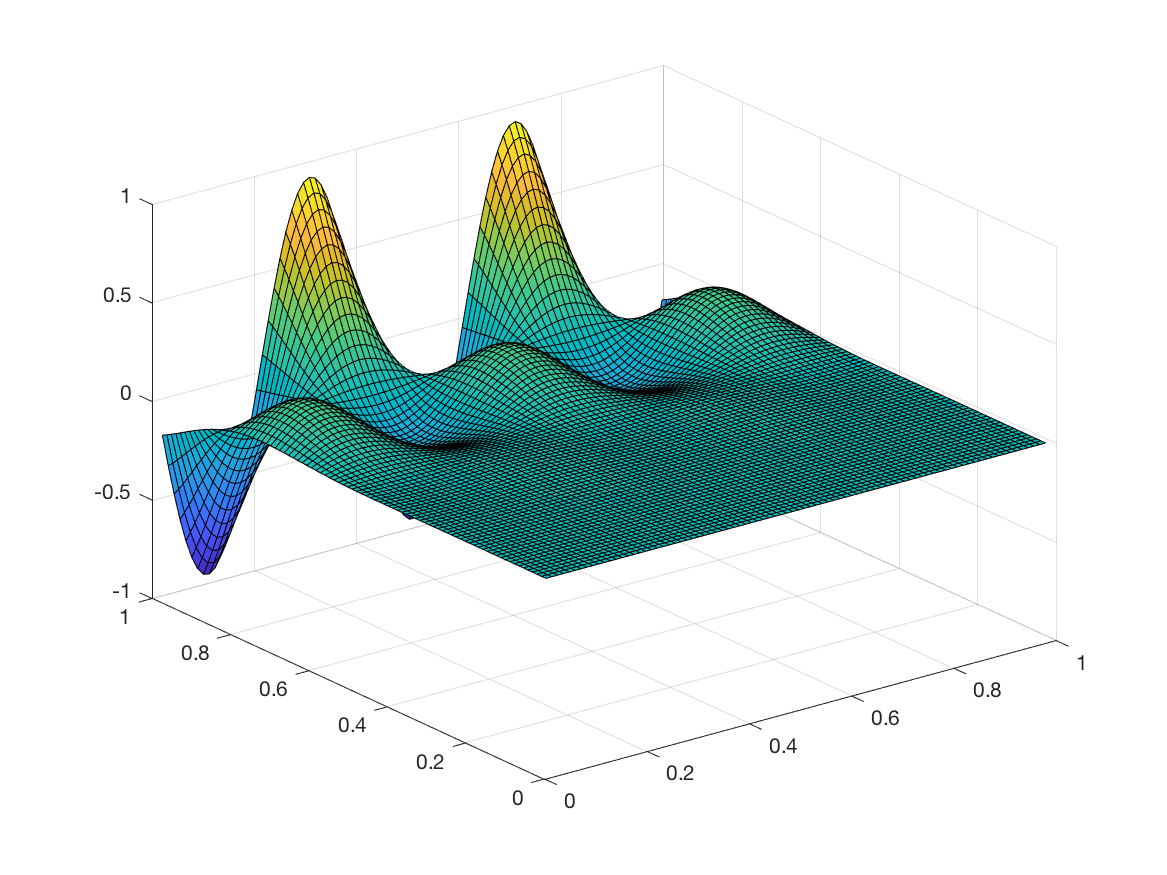
\includegraphics[width=\linewidth]{../Figures/poisson_approx_5.png}\\\hline
  \end{tabular}
\end{center}

\newpage
\newquestion
%======================================================
%
%                    Problem 2
%
%======================================================
\section*{Problem 2}

\newpart
%--------------------------
%    Problem 2 Part A
%--------------------------
\subsection*{(a)}
The centered-difference approximation for the partial difference equations has the form:
\begin{eqnarray*}
  \frac{2v_{j,k}-v_{j-1,k}-v_{j+1,k}}{h_x^2}+\frac{2v_{j,k}-v_{j,k-1}-v_{j,k+1}}{h_y^2}+\sigma v_{j,k}&=&f\left(x_j,y_k\right)\\
  \frac{1}{h_x^2}T_{m_x}V+\frac{1}{h_y^2}VT_{m_y}-\frac{1}{h_x^2}B-\frac{1}{h_y^2}C+\sigma V&=&F\\
  T_{m_x}V+\frac{h_x^2}{h_y^2}VT_{m_y}+h_x^2\sigma V&=&h_x^2\left(F+\frac{1}{h_x^2}B+\frac{1}{h_y^2}C\right)\\
  T_{m_x}V+\alpha VT_{m_y}+\beta V&=&\tilde{F}
\end{eqnarray*}
where
\begin{align*}
  \alpha&=\left(\frac{h_x}{h_y}\right)^2&\beta&=h_x^2\sigma\\
  \tilde{F}&=h_x^2\left(F+\frac{1}{h_x^2}B+\frac{1}{h_y^2}C\right)\\
  B&=\left[
  \begin{array}{cccc}
    b_{01}&b_{02}&\cdots&b_{0m}\\
    0&0&\cdots&0\\
    \vdots&\vdots&&\vdots\\
    0&0&\cdots&0\\
    b_{11}&b_{12}&\cdots&b_{1m}\\
  \end{array}
  \right]\qquad &C&=\left[
  \begin{array}{ccccc}
    c_{01}&0&\cdots&0&c_{11}\\
    c_{02}&0&\cdots&0&c_{12}\\
    \vdots&\vdots&&\vdots&\vdots\\
    c_{0m}&0&\cdots&0&c_{1m}\\
  \end{array}
  \right]\\
  b_{0j}&=g\left(x_j,0\right)&c_{0k}&=g\left(0,y_k\right)\\
  b_{1j}&=g\left(x_j,b\right)&c_{1k}&=g\left(a,y_k\right)
\end{align*}

\newpart
%--------------------------
%    Problem 2 Part B
%--------------------------
\subsection*{(b)}
\begin{eqnarray*}
  T_{m_x}V+\alpha VT_{m_y}+\beta V&=&\tilde{F}\\
  Z_{m_x}^TT_{m_x}Z_{m_x}Z_{m_x}^TVZ_{m_y}+Z_{m_x}^TVZ_{m_y}Z_{m_y}^TVZ_{m_y}+\beta Z_{m_x}^TVZ_{m_y}&=&Z_{m_x}^T\tilde{F}Z_{m_y}^T\\
  \Lambda_{m_x} V'+\alpha V'\Lambda_{m_y}+\beta V'&=&\tilde{F}'\\
  \lambda_j v_{jk}'+\alpha v_{jk}'\lambda_k+\beta v_{jk}'&=&\tilde{f}_{jk}'\\
  v_{jk}'&=&\frac{\tilde{f_{jk}}'}{\lambda_{j}+\alpha \lambda_k+\beta}\\
  V&=&Z_{m_x}^TV'Z_{m_y}
\end{eqnarray*}
The number of flops would be of order $\mathcal{O}\left(m_xm_y\log\left(m_x\right)+m_ym_x\log\left(m_x\right)\right)=\mathcal{O}\left(m_xm_y\log\left(m_xm_y\right)\right)$.

\newpage
\newquestion
%======================================================
%
%                    Problem 3
%
%======================================================
\section*{Problem 3}
Let $c=\left[c_0,c_1,c_2,\dots,c_{n-1}\right]^T$.
The Frobenius norm can be written as
\begin{eqnarray*}
  \norm{C-T}_F&=&\textrm{trace}\left(\left(C-T\right)^T\left(C-T\right)\right)\\
              &=&\textrm{trace}\left(\left(C^T-T^T\right)\left(C-T\right)\right)\\
              &=&\textrm{trace}\left(C^TC-C^TT-T^TC-T^TT\right)
\end{eqnarray*}
Thus,
\begin{eqnarray*}
  P=\left[p_{ij}\right]_{i,j=0,\dots,n-1}&=&C^TC\\
                              &=&\left[
                                  \begin{array}{ccccc}
                                    c_0&c_{n-1}&c_{n-2}&\cdots&c_1\\
                                    c_1&c_0&c_{n-1}&\cdots&c_2\\
                                    c_2&c_1&c_0&\cdots&c_3\\
                                    \vdots&\vdots&\vdots&\ddots&\vdots\\
                                    c_{n-1}&c_{n-2}&c_{n-3}&\cdots&c_0\\
                                  \end{array}
  \right]\left[
  \begin{array}{ccccc}
    c_0&c_1&c_2&\cdots&c_{n-1}\\
    c_{n-1}&c_0&c_1&\cdots&c_{n-2}\\
    c_{n-2}&c_{n-1}&c_0&\cdots&c_{n-3}\\
    \vdots&\vdots&\vdots&\ddots&\vdots\\
    c_1&c_2&c_3&\cdots&c_0\\
  \end{array}
  \right]\\
  p_{ii}&=&c_i^2+c_{i-1}^2+\cdots+c_1^2+c_0^2+c_{n-1}^2+c_{n-2}^2+\cdots+c_{i+1}^2\\
                              &=&c^Tc\\
  \textrm{trace}\left(P\right)&=&\sum_{i=0}^{n-1}p_{ii}\\
                              &=&nc^Tc
\end{eqnarray*}
\begin{eqnarray*}
  Q=\left[q_{ij}\right]_{i,j=0,\dots,n-1}&=&C^TT\\
                                         &=&\left[
                                             \begin{array}{ccccc}
                                               c_0&c_{n-1}&c_{n-2}&\cdots&c_1\\
                                               c_1&c_0&c_{n-1}&\cdots&c_2\\
                                               c_2&c_1&c_0&\cdots&c_3\\
                                               \vdots&\vdots&\vdots&\ddots&\vdots\\
                                               c_{n-1}&c_{n-2}&c_{n-3}&\cdots&c_0\\
                                             \end{array}
  \right]\left[
  \begin{array}{ccccc}
    t_0&t_1&t_2&\cdots&t_{n-1}\\
    t_1&t_0&t_1&\cdots&t_{n-2}\\
    t_2&t_1&t_0&\cdots&t_{n-3}\\
    \vdots&\vdots&\vdots&\ddots&\vdots\\
    t_{n-1}&t_{n-2}&t_{n-3}&\cdots&t_0\\
  \end{array}
  \right]\\
  q_{ii}&=&c_it_i+c_{i-1}t_{i-1}+\cdots+c_1t_1+c_0t_0+c_{n-1}t_1+c_{n-2}t_2+\cdots+c_{i+1}t_{n-i-1}\\
                                         &=&\sum_{k=0}^ic_{i-k}t_{i-k}+\sum_{k=1}^{n-i-1}c_{n-k}t_k\\
  \textrm{trace}\left(Q\right)&=&\sum_{i=0}^{n-1}q_{ii}\\
                                         &=&\sum_{i=0}^{n-1}\left(\sum_{k=0}^ic_{i-k}t_{i-k}+\sum_{k=1}^{n-i-1}c_{n-k}t_k\right)
\end{eqnarray*}
Similarly,
\begin{eqnarray*}
  R=\left[r_{ij}\right]_{i,j=0,\dots,n-1}&=&T^TC\\
                                         &=&\left[
                                             \begin{array}{ccccc}
                                               t_0&t_1&t_2&\cdots&t_{n-1}\\
                                               t_1&t_0&t_1&\cdots&t_{n-2}\\
                                               t_2&t_1&t_0&\cdots&t_{n-3}\\
                                               \vdots&\vdots&\vdots&\ddots&\vdots\\
                                               t_{n-1}&t_{n-2}&t_{n-3}&\cdots&t_0\\
                                             \end{array}
  \right]\left[
  \begin{array}{ccccc}
    c_0&c_1&c_2&\cdots&c_{n-1}\\
    c_{n-1}&c_0&c_1&\cdots&c_{n-2}\\
    c_{n-2}&c_{n-1}&c_0&\cdots&c_{n-3}\\
    \vdots&\vdots&\vdots&\ddots&\vdots\\
    c_1&c_2&c_3&\cdots&c_0\\
  \end{array}
  \right]\\
  r_{ii}&=&t_ic_i+t_{i-1}c_{i-1}+\cdots+t_1c_1+t_0c_0+t_1c_1+t_2c_2+\cdots+t_{n-i-1}c_{n-i-1}\\
                                         &=&\sum_{k=0}^it_{i-k}c_{i-k}+\sum_{k=1}^{n-i-1}t_{k}c_k\\
  \textrm{trace}\left(R\right)&=&\sum_{i=0}^{n-1}r_{ii}\\
                                         &=&\sum_{i=0}^{n-1}\left(\sum_{k=0}^it_{i-k}c_{i-k}+\sum_{k=1}^{n-i-1}t_kc_k\right)
\end{eqnarray*}
Thus, $\textrm{trace}\left(Q\right)=\textrm{trace}\left(R\right)$. Let $\nabla=\left[\frac{\partial}{\partial c_1},\dots,\frac{\partial}{\partial c_{n-1}}\right]$. To minimize $\norm{C-T}_F$, set
\begin{eqnarray*}
  \left(\nabla\norm{C-T}_F\right)_{j}&=&\frac{\partial}{\partial c_j}\textrm{trace}\left(C^TC-C^TT-T^TC-T^TT\right)\\
                                     &=&\frac{\partial}{\partial c_j}\left[\sum_{k=0}^{n-1}c_k^2-2\sum_{i=0}^{n-1}\left(\sum_{k=0}^ic_{i-k}t_{i-k}+\sum_{k=1}^{n-i-1}c_{n-k}t_k\right)\right]\\
                                     &=&2nc_j-2\left[\left(n-j\right)t_j+jt_{n-j}\right]\\
                                     &=&0\\
  c_j&=&\frac{1}{n}\left[\left(n-j\right)t_j+jt_{n-j}\right]
\end{eqnarray*}
Since there is only one solution to $\nabla\norm{C-T}_F=0$, then $C_T$ is unique. Also, since
\begin{eqnarray*}
  c_{n-j}&=&\frac{1}{n}\left[\left(n-\left(n-j\right)\right)t_{n-j}+\left(n-j\right)t_{n-\left(n-j\right)}\right]\\
     &=&\frac{1}{n}\left[jt_{n-j}+\left(n-j\right)t_j\right]\\
     &=&c_j,
\end{eqnarray*}
then $c_j$ is symmetric.

\newpage
\newquestion
%======================================================
%
%                    Problem 4
%
%======================================================
\section*{Problem 4}

\newpart
%--------------------------
%    Problem 4 Part A
%--------------------------
\subsection*{(a)}
\lstinputlisting[style=Matlab-editor,basicstyle=\ttfamily\small]{../Code/toeplitzpcg.m}

\newpart
%--------------------------
%    Problem 4 Part B
%--------------------------
\subsection*{(b)}
\lstinputlisting[style=Matlab-editor,basicstyle=\ttfamily\small]{../Code/toeplitzpcgcirc.m}

\newpage
\newpart
%--------------------------
%    Problem 4 Part C
%--------------------------
\subsection*{(c)}
\lstinputlisting[style=Matlab-editor,basicstyle=\ttfamily\small]{../Code/homework3_4_c_1.m}
\newpage
For $n=10$, the output is,

\begin{tabular}{c|c|c}
  $p=1$&$p=0.1$&$p=0.01$\\\hline
  \multicolumn{3}{c}{without preconditioning}\\\hline
  $\left[\begin{array}{r}
\texttt{3.450926863794943e-01}\\
\texttt{2.428161529760083e-01}\\
\texttt{2.061924099579956e-01}\\
\texttt{1.896360060540769e-01}\\
\texttt{1.828445601954354e-01}\\
\texttt{1.828445601954350e-01}\\
\texttt{1.896360060540770e-01}\\
\texttt{2.061924099579958e-01}\\
\texttt{2.428161529760081e-01}\\
\texttt{3.450926863794944e-01}\\
\end{array}
\right]$&$\left[\begin{array}{r}
\texttt{1.975370703537823e-01}\\
\texttt{1.138792774427789e-01}\\
\texttt{8.775407132745998e-02}\\
\texttt{7.691072994649119e-02}\\
\texttt{7.265683421537614e-02}\\
\texttt{7.265683421537471e-02}\\
\texttt{7.691072994648715e-02}\\
\texttt{8.775407132745379e-02}\\
\texttt{1.138792774427705e-01}\\
\texttt{1.975370703537805e-01}\\
\end{array}
\right]$&$\left[\begin{array}{r}
\texttt{1.857935191671665e-01}\\
\texttt{1.045415317727272e-01}\\
\texttt{7.961205681990180e-02}\\
\texttt{6.937790019383741e-02}\\
\texttt{6.538557146064886e-02}\\
\texttt{6.538557146065589e-02}\\
\texttt{6.937790019375377e-02}\\
\texttt{7.961205681977551e-02}\\
\texttt{1.045415317726247e-01}\\
\texttt{1.857935191670622e-01}\\
\end{array}
\right]$\\\hline
  \multicolumn{3}{c}{with preconditioning}\\\hline
  $\left[\begin{array}{r}
\texttt{3.450926863795118e-01}\\
\texttt{2.428161529760274e-01}\\
\texttt{2.061924099580156e-01}\\
\texttt{1.896360060540973e-01}\\
\texttt{1.828445601954564e-01}\\
\texttt{1.828445601954559e-01}\\
\texttt{1.896360060540976e-01}\\
\texttt{2.061924099580162e-01}\\
\texttt{2.428161529760276e-01}\\
\texttt{3.450926863795120e-01}\\
\end{array}
\right]$&$\left[\begin{array}{r}
\texttt{1.975370703537795e-01}\\
\texttt{1.138792774427788e-01}\\
\texttt{8.775407132745931e-02}\\
\texttt{7.691072994648539e-02}\\
\texttt{7.265683421537593e-02}\\
\texttt{7.265683421537601e-02}\\
\texttt{7.691072994648594e-02}\\
\texttt{8.775407132745613e-02}\\
\texttt{1.138792774427781e-01}\\
\texttt{1.975370703537801e-01}\\
\end{array}
\right]$&$\left[\begin{array}{r}
\texttt{1.857935201528620e-01}\\
\texttt{1.045415204154867e-01}\\
\texttt{7.961210248459726e-02}\\
\texttt{6.937782132363908e-02}\\
\texttt{6.538561503746061e-02}\\
\texttt{6.538561503743219e-02}\\
\texttt{6.937782132361736e-02}\\
\texttt{7.961210248460469e-02}\\
\texttt{1.045415204154808e-01}\\
\texttt{1.857935201529732e-01}\\
\end{array}
\right]$\\
\end{tabular}

For $n=100$, the output is,

\begin{tabular}{c|c|c}
  &$p=1$&$p=0.1$\\\hline
  \multicolumn{3}{c}{without preconditioning}\\\hline
  $\left[
  \begin{array}{c}
    x(1)\\
    x(100000)\\
    x(500000)\\
    x(700000)\\
    x(1000000)
  \end{array}
  \right]$&$\left[\begin{array}{r}
\texttt{1.676284540637890e-02}\\
\texttt{4.147019469754698e-04}\\
\texttt{3.202634777824108e-04}\\
\texttt{3.346753478040451e-04}\\
\texttt{1.676284540576385e-02}\\
\end{array}
\right]$&$\left[\begin{array}{r}
\texttt{9.532317527874454e-04}\\
\texttt{1.985347566261856e-06}\\
\texttt{1.221933191103328e-06}\\
\texttt{1.327454413917721e-06}\\
\texttt{9.532317519653615e-04}\\
\end{array}
\right]$\\\hline
  \multicolumn{3}{c}{with preconditioning}\\\hline
  $\left[\begin{array}{c}
           x(1)\\
           x(100000)\\
           x(500000)\\
           x(700000)\\
           x(1000000)
         \end{array}
  \right]$&$\left[\begin{array}{r}
\texttt{1.676284622516175e-02}\\
\texttt{4.147019516876527e-04}\\
\texttt{3.202634824103388e-04}\\
\texttt{3.346753506434133e-04}\\
\texttt{1.676284622546426e-02}\\
\end{array}
\right]$&$\left[\begin{array}{r}
\texttt{9.532780564171566e-04}\\
\texttt{1.985338116172135e-06}\\
\texttt{1.221936166062850e-06}\\
\texttt{1.327449171076912e-06}\\
\texttt{9.532780564631677e-04}\\
\end{array}
\right]$\\
\end{tabular}

\newpage
\newquestion
%======================================================
%
%                    Problem 5
%
%======================================================
\section*{Problem 5}

\newpart
%--------------------------
%    Problem 5 Part A
%--------------------------
\subsection*{(a)}
\lstinputlisting[style=Matlab-editor,basicstyle=\ttfamily\small]{../Code/get_lower.m}

\newpart
%--------------------------
%    Problem 5 Part B
%--------------------------
\subsection*{(b)}
\lstinputlisting[style=Matlab-editor,basicstyle=\ttfamily\small]{../Code/iCholesky.m}

\newpage
\newpart
%--------------------------
%    Problem 5 Part C
%--------------------------
\subsection*{(c)}
\lstinputlisting[style=Matlab-editor,basicstyle=\ttfamily\small]{../Code/solve_lower.m}

\newpart
%--------------------------
%    Problem 5 Part D
%--------------------------
\subsection*{(d)}
\lstinputlisting[style=Matlab-editor,basicstyle=\ttfamily\small]{../Code/solve_lowert.m}

\newpage
\newpart
%--------------------------
%    Problem 5 Part E
%--------------------------
\subsection*{(e)}
\lstinputlisting[style=Matlab-editor,basicstyle=\ttfamily\small]{../Code/homework3_5_e_1.m}

\newpage
The small matrix had the following output.

\begin{tabular}{c|c|c}
  &without preconditioning & with preconditioning\\\hline
  iterations&13&11\\\hline
  $\frac{\norm{Ax-b}_2}{\norm{b_2}}$&\texttt{4.668821516582010e-16}&\texttt{3.024858452994199e-10}\\\hline
  $x$ & $\left[\begin{array}{r}
\texttt{-4.615232329669224e-02}\\
\texttt{5.560346406107559e-02}\\
\texttt{4.674441847347385e-01}\\
\texttt{1.436167453017343e-01}\\
\texttt{-2.747396794324581e+00}\\
\texttt{-9.595158505895890e-01}\\
\texttt{-5.588795197458957e-01}\\
\texttt{-5.625708181717426e-01}\\
\texttt{4.963846660536811e-01}\\
\texttt{4.553705821620747e-01}\\
\texttt{-8.540096449002311e-01}\\
\texttt{1.546983563153979e-01}\\
\texttt{7.076179967126332e-02}\\
\texttt{-7.644048349576092e-02}\\
\texttt{-2.310798723702473e+00}\\
\texttt{-1.815291036261631e+00}\\
\texttt{-1.576605857315947e+00}\\
\texttt{-2.519078345042125e+00}\\
\texttt{-9.076946955455132e-01}\\
\texttt{-1.120184575920670e+00}\\
\texttt{-1.946389613822066e-01}\\
\texttt{1.198432367141279e-01}\\
\texttt{-1.119327367250933e+00}\\
\texttt{-3.088950654587257e+00}\\
\texttt{-7.670423173687755e-01}\\
\end{array}
\right]$ & $\left[\begin{array}{r}
\texttt{-4.615232331993605e-02}\\
\texttt{5.560346408639215e-02}\\
\texttt{4.674441847709141e-01}\\
\texttt{1.436167453602924e-01}\\
\texttt{-2.747396794334826e+00}\\
\texttt{-9.595158508044294e-01}\\
\texttt{-5.588795196477444e-01}\\
\texttt{-5.625708181081200e-01}\\
\texttt{4.963846659080517e-01}\\
\texttt{4.553705824433909e-01}\\
\texttt{-8.540096447547476e-01}\\
\texttt{1.546983564603329e-01}\\
\texttt{7.076179962288556e-02}\\
\texttt{-7.644048328883853e-02}\\
\texttt{-2.310798723518883e+00}\\
\texttt{-1.815291036181375e+00}\\
\texttt{-1.576605856924276e+00}\\
\texttt{-2.519078344987517e+00}\\
\texttt{-9.076946956506157e-01}\\
\texttt{-1.120184576068447e+00}\\
\texttt{-1.946389613226679e-01}\\
\texttt{1.198432364684508e-01}\\
\texttt{-1.119327367504965e+00}\\
\texttt{-3.088950654440442e+00}\\
\texttt{-7.670423169847281e-01}\\
\end{array}
\right]$
\end{tabular}
\newpage
The vectors $J$, $I$, and $V_L$ correspond to the CSC format of the incomplete Cholesky factorization of $A$ and were reshaped to fit onto the page.
\begin{eqnarray*}
  J&=&\left[\begin{array}{rrr}
\texttt{1}&\texttt{7}&\texttt{18}\\
\texttt{2}&\texttt{21}&\texttt{23}\\
\texttt{9}&\texttt{24}&\texttt{24}\\
\texttt{21}&\texttt{8}&\texttt{16}\\
\texttt{2}&\texttt{11}&\texttt{17}\\
\texttt{6}&\texttt{23}&\texttt{20}\\
\texttt{7}&\texttt{9}&\texttt{17}\\
\texttt{3}&\texttt{13}&\texttt{19}\\
\texttt{10}&\texttt{10}&\texttt{21}\\
\texttt{20}&\texttt{16}&\texttt{24}\\
\texttt{4}&\texttt{22}&\texttt{18}\\
\texttt{6}&\texttt{11}&\texttt{25}\\
\texttt{7}&\texttt{12}&\texttt{19}\\
\texttt{8}&\texttt{14}&\texttt{20}\\
\texttt{15}&\texttt{25}&\texttt{20}\\
\texttt{5}&\texttt{13}&\texttt{21}\\
\texttt{16}&\texttt{19}&\texttt{22}\\
\texttt{18}&\texttt{21}&\texttt{25}\\
\texttt{22}&\texttt{14}&\texttt{23}\\
\texttt{24}&\texttt{18}&\texttt{24}\\
\texttt{6}&\texttt{23}&\texttt{25}\\
\texttt{11}&\texttt{15}&\texttt{NaN}\\
\end{array}
\right]\qquad I=\left[\begin{array}{rr}
\texttt{1}&\texttt{41}\\
\texttt{5}&\texttt{44}\\
\texttt{8}&\texttt{48}\\
\texttt{11}&\texttt{51}\\
\texttt{16}&\texttt{55}\\
\texttt{21}&\texttt{57}\\
\texttt{23}&\texttt{59}\\
\texttt{26}&\texttt{60}\\
\texttt{29}&\texttt{61}\\
\texttt{31}&\texttt{63}\\
\texttt{34}&\texttt{64}\\
\texttt{35}&\texttt{65}\\
\texttt{38}&\texttt{66}\\
\end{array}
\right]\\
  V_L&=&\left[\begin{array}{rrr}
\texttt{2.000000000000000e+00}&\texttt{1.866369023889256e+00}&\texttt{-5.163977794943222e-01}\\
\texttt{-5.000000000000000e-01}&\texttt{-5.357997197768198e-01}&\texttt{-5.163977794943222e-01}\\
\texttt{-5.000000000000000e-01}&\texttt{-5.357997197768198e-01}&\texttt{-5.163977794943222e-01}\\
\texttt{-5.000000000000000e-01}&\texttt{1.936491673103709e+00}&\texttt{1.866369023889256e+00}\\
\texttt{1.936491673103709e+00}&\texttt{-5.163977794943222e-01}&\texttt{-5.357997197768198e-01}\\
\texttt{-5.163977794943222e-01}&\texttt{-5.163977794943222e-01}&\texttt{-5.357997197768198e-01}\\
\texttt{-5.163977794943222e-01}&\texttt{1.936491673103709e+00}&\texttt{1.926893525934186e+00}\\
\texttt{2.000000000000000e+00}&\texttt{-5.163977794943222e-01}&\texttt{-5.189700346910373e-01}\\
\texttt{-5.000000000000000e-01}&\texttt{1.936491673103709e+00}&\texttt{-5.189700346910373e-01}\\
\texttt{-5.000000000000000e-01}&\texttt{-5.163977794943222e-01}&\texttt{-5.189700346910373e-01}\\
\texttt{2.000000000000000e+00}&\texttt{-5.163977794943222e-01}&\texttt{1.793506806975281e+00}\\
\texttt{-5.000000000000000e-01}&\texttt{1.856408358530099e+00}&\texttt{-5.575668829974966e-01}\\
\texttt{-5.000000000000000e-01}&\texttt{2.000000000000000e+00}&\texttt{1.860863498549972e+00}\\
\texttt{-5.000000000000000e-01}&\texttt{-5.000000000000000e-01}&\texttt{-5.373849295121450e-01}\\
\texttt{-5.000000000000000e-01}&\texttt{-5.000000000000000e-01}&\texttt{1.781610534830862e+00}\\
\texttt{2.000000000000000e+00}&\texttt{1.932183566158592e+00}&\texttt{1.710477015490919e+00}\\
\texttt{-5.000000000000000e-01}&\texttt{-5.175491695067657e-01}&\texttt{1.866369023889256e+00}\\
\texttt{-5.000000000000000e-01}&\texttt{-5.175491695067657e-01}&\texttt{-5.357997197768198e-01}\\
\texttt{-5.000000000000000e-01}&\texttt{1.936491673103709e+00}&\texttt{1.788854381999832e+00}\\
\texttt{-5.000000000000000e-01}&\texttt{-5.163977794943222e-01}&\texttt{1.710824975476217e+00}\\
\texttt{1.866369023889256e+00}&\texttt{-5.163977794943222e-01}&\texttt{1.775397936033366e+00}\\
\texttt{-5.357997197768198e-01}&\texttt{1.936491673103709e+00}&\texttt{NaN}\\
\end{array}
\right]
\end{eqnarray*}
\newpage
The large matrix had the following output where $J$, $I$, and $V_L$ correspond to CSC format of the the incoomplete Cholesky factorization.

\begin{tabular}{c|c|c}
  &without preconditioning & with preconditioning\\\hline
  iterations&249&111\\\hline
  $
  \begin{array}{c}
          x\left(1\right)\\
          x\left(10000\right)\\
          x\left(100000\right)\\
          x\left(200000\right)\\
          x\left(262144\right)\\
  \end{array}$ & $\begin{array}{r}
\texttt{4.286321404907984e-01}\\
\texttt{7.121924304536499e-01}\\
\texttt{-2.453852875592730e+00}\\
\texttt{-2.497480687000048e+00}\\
\texttt{1.938920155215448e+00}\\
\end{array}
$ & $\begin{array}{r}
\texttt{4.286321980474398e-01}\\
\texttt{7.121923784405517e-01}\\
\texttt{-2.453852852351424e+00}\\
\texttt{-2.497480719783645e+00}\\
\texttt{1.938920151693724e+00}\\
\end{array}
$
\end{tabular}

\begin{tabular}{c|c|c|c}
  index & $J$ & $I$ & $V_L$\\\hline
  $
  \begin{array}{r}
    1\\
    10\\
    100\\
    1000\\
    \texttt{end}
  \end{array}
$ & $\begin{array}{r}
\texttt{1}\\
\texttt{45882}\\
\texttt{132301}\\
\texttt{102399}\\
\texttt{262144}\\
\end{array}
$ & $\begin{array}{r}
\texttt{1}\\
\texttt{63}\\
\texttt{685}\\
\texttt{6887}\\
\texttt{1036289}\\
\end{array}
$ & $\begin{array}{r}
\texttt{2.449489742783178e+00}\\
\texttt{-4.082482904638631e-01}\\
\texttt{-4.082482904638631e-01}\\
\texttt{-4.082482904638631e-01}\\
\texttt{2.220117073041080e+00}\\
\end{array}
$
\end{tabular}

\end{document}
%================================================================
%================================================================
%
%                           Templates
%
%================================================================
%================================================================


%----------------------------------------------------------------
%----------------------------------------------------------------


\newquestion
%======================================================
%
%                    Problem n
%
%======================================================
\section*{Problem n}

\newpart
%--------------------------
%    Problem n Part A
%--------------------------
\subsection*{(a)}

\newpart
%--------------------------
%    Problem n Part B
%--------------------------
\subsection*{(b)}


%----------------------------------------------------------------
%----------------------------------------------------------------


%======================================================
%
%               Appendix: Problem n
%
%======================================================
%--------------------------
%  Appendix: P n Part A
%--------------------------
\subsection*{Problem n Part A}

\newpage
%--------------------------
%  Appendix: P n Part B
%--------------------------
\subsection*{Problem n Part B}


%----------------------------------------------------------------
%----------------------------------------------------------------